\chapter{Packages and Programs}
\label{package}

\lettrine[nindent=0.1em]{A}{lthough it may seem} that programming is \emph{all about algorithms}, in practice algorithms make up only a small portion of a programmer's task. By far the largest part of a programmer's job revolves around structure and organization. \go language structures revolve around three principal constructs: rules, classes and packages -- in increasing order of granularity. 

In this chapter we focus on this larger scale aspects of \go programs -- namely \firstterm{package}{A package is a group of related definitions and programs that is compiled and loaded as a single unit. Packages may contain variables, classes, rules and types. Packages are accessed with the \q{import} statement.}s -- which are \go's equivalent of modules.

\go has a simple but effective package system that allows programs, classes and types to be defined in one file and re-used in others. A top-level program also takes the form of a package -- with the addition of a standard action rule defined for the \q{main} symbol.

Packages may \q{import} other packages, with no limit except that the \q{import} chains should not be circular. Imported packages are loaded automatically whenever the referring package is loaded. However many times a package is \q{import}ed, it will only ever be loaded once.

\section{Package format}
\label{package:format}
\index{format of a package}
\index{package!format}
\index{modules!go@\go packages}
Each \go source file makes up a single package. The form of a package file is:
\begin{alltt}
\emph{packagename}\{
  \ldots
  \emph{Definitions}
  \ldots
\}
\end{alltt}
\index{package!file names of packages}
The \emph{packagename} is either a single identifier, or a sequence of identifiers separated by periods.

\index{package!name}
\index{name of package}
\index{files and packages}
Note that the \emph{packagename} must reflect the name of the file containing it. For example, if the package name is 
\begin{alltt}
foo.bar
\end{alltt}
then the \emph{name} of the file containing this package should be of the form:
\begin{alltt}
\ldots/foo/bar.go
\end{alltt}
i.e., the package source file must be located in a particular directory structure -- to the extent that the package name requires it.
\begin{aside}
The \emph{reason} for this is that the \go engine has to be able to locate the file containing the compiled package when it is loaded.
\end{aside}

\index{contents of a package}
A package may contain class definitions, rule definitions, type definitions, package variable definitions, package constant definitions and initialization actions. It may also include directives to \q{import} other packages. 

\index{order of definitions}
\index{package!order of definitions in}
The order of definitions within a package is not important -- the \go compiler is able to handle mutually recursive programs without requiring forward declarations. Many of the elements in a package are defined elsewhere in this manual. In the following sections we focus on those elements that are not covered elsewhere.

\subsection{Package constants}
\label{package:constant}
\index{constants in packages}
\index{package!constant in}
\index{operator!=@\q{=}}

A package constant is declared at the top-level of a package, using a \q{=} statement:
\begin{alltt}
\emph{packageName}\{
  \ldots
  V:\emph{type} = \emph{value}
  \ldots
\}
\end{alltt}
The identifier \q{V} is constant in the sense that, once \q{\emph{value}} is evaluated and bound to \q{V}, it is not modifiable. It is evaluated as the package is loaded, in an order that is not guaranteed -- although the compiler ensures that any dependent values are evaluated before the variable itself is evaluated.

Unlike package variables (see below), by default package constants \emph{are} exported from a package. Thus constants declared in a package are made available to any packages that \q{import} the package.

Package constants -- and package variables -- may only be bound to \emph{ground} values.

\subsection{Package variables}
\label{package:variable}
\index{variable!in packages}
\index{package!variables in}
\index{operator!:=@\q{:=}}

A package variable is a re-assignable variable declared at the top-level of a package, using a \q{:=} statement:
\begin{alltt}
\emph{packageName}\{
  \ldots
  V:\emph{type} := \emph{initial}
  \ldots
\}
\end{alltt}
Package variables have two major restrictions -- compared to regular logic variables -- their values must be ground at all times; in addition, package variables are not exportable from packages. They also have a major liberation -- they can be re-assigned.


\begin{aside}
Package constants and variables are evaluated in the full context of the package; i.e., the expressions that define their value can involve functions defined in the package and can even involve -- directly or indirectly -- other package constants and variables.

The compiler will not necessarily respect the order of occurrence of package constants and variables in the file: they will be evaluated \emph{after} evaluating any constants and variables that they depend on. However, if there is a circular dependency between package constants/variables; if the expression denoting the value of a constant refers to another constant, \emph{and} that constant's value expression also refers to this constant, then there is  a circular dependency between the two variables. This can lead to serious problems when loading the package -- it is possible for the \go system to enter into a loop \emph{during the loading} of the module.

As a result, it is recommended to avoid circular dependencies amongst package constants and variables.

This does not apply to mutually recursive programs however; as they are not evaluated as part of the package loading process. Therefore, it is quite safe to have mutually recursive programs. Furthermore, those mutually recursive programs may reference package variables and constants without harm.
\end{aside}

\begin{aside}
Most importantly, if two packages are \q{import}ed independently, there is no pre-defined order of \q{import}ing, and hence the order of evaluation of package constants in different packages is not defined.
\end{aside}

\subsection{Package initialization}
\label{package:initialization}
\index{evaluation order!in packages}

In addition to package variables and constants having an initial expression associated with them, it is possible to define an action that will be executed on loading the package. Such initialization actions use the notation:
\begin{alltt}
\emph{packageName}\{
  \ldots
  \$ \{
    \emph{Action}
  \}
  \ldots
\}
\end{alltt}
The initialization action is executed \emph{after} any initializers associated with package constants and variables. Furthermore, if a package \q{imports} one or more other packages, then the initializers of those packages will also be run before the importing package's initializer -- thus ensuring that the initializer executes in a well defined environment.

A package can have any number of initializers in its body, however the relative order of execution between these different initializers is not defined.

Package initializers can be useful for certain classes of \emph{active} packages -- such as file system packages that may need to open certain standard files. For example, the \q{go.io} standard package has an initializer that opens the three standard files: \q{stdout}, \q{stdin} and \q{stderr}.

\begin{aside}
If a package initializer, or a variable or constant initializer, \q{raise}s an unrecovered exception then the entire package loading process will \emph{abort} and the \go session will terminate.
\end{aside}

\subsection{Package exports}
\label{package:export}

The elements exported by the package include any rule programs (functions, relation definitions etc.), classes \emph{and types}. By default, \emph{all} the elements defined in a package are exported; except for re-assignable package variables. However, a definition may be prefixed by the \q{private} keyword, in which case the definition will not be exported.
\index{keyword!private@\q{private}}
\begin{aside}
Note that package variables -- as opposed to package constants -- are not made available to importing packages. If it is important that an updateable variable is exported then it should be wrapped with accessor programs that can be used to set the variable and to get its value:
\index{operator!:=@\q{:=}}
\begin{alltt}
export\{
  V:\emph{type} := \emph{Init}.  -- we are going to 'export' V
  
  setV:[\emph{type}]*.
  setV(N) -> V := N.
    
  getV:[]=>\emph{type}.
  getV() => V.
\}
\end{alltt}
\end{aside}

\section{Importing packages}
\label{package:import}
\index{importing packages}
\index{package!importing of}
\index{import@\q{import} directive}
\index{keyword!import@\q{import}}
The \q{import} directive in a package body is used to indicate that a particular package is required for that package. The form of the \q{import} statement is:
\begin{alltt}
import \emph{packagename}.
\end{alltt}
where \emph{packagename} is a dotted sequence of identifiers that matches the package name used in the package file. 

The effect of an \q{import} directive is to make available to the importing package all the definitions of the imported package. This includes classes, rules of various kinds, any types defined within the imported package and any \emph{constants} defined within the package.

The \go engine ensures that any given package will only be loaded once, however many requests for its \q{import} are found. Furthermore, any initialization code associated with a package (see \vref{package:initialization}) will also only be executed once.

\subsection{Indirect \q{import}s of packages}
\index{package!indirect \q{import}}
\begin{figure}
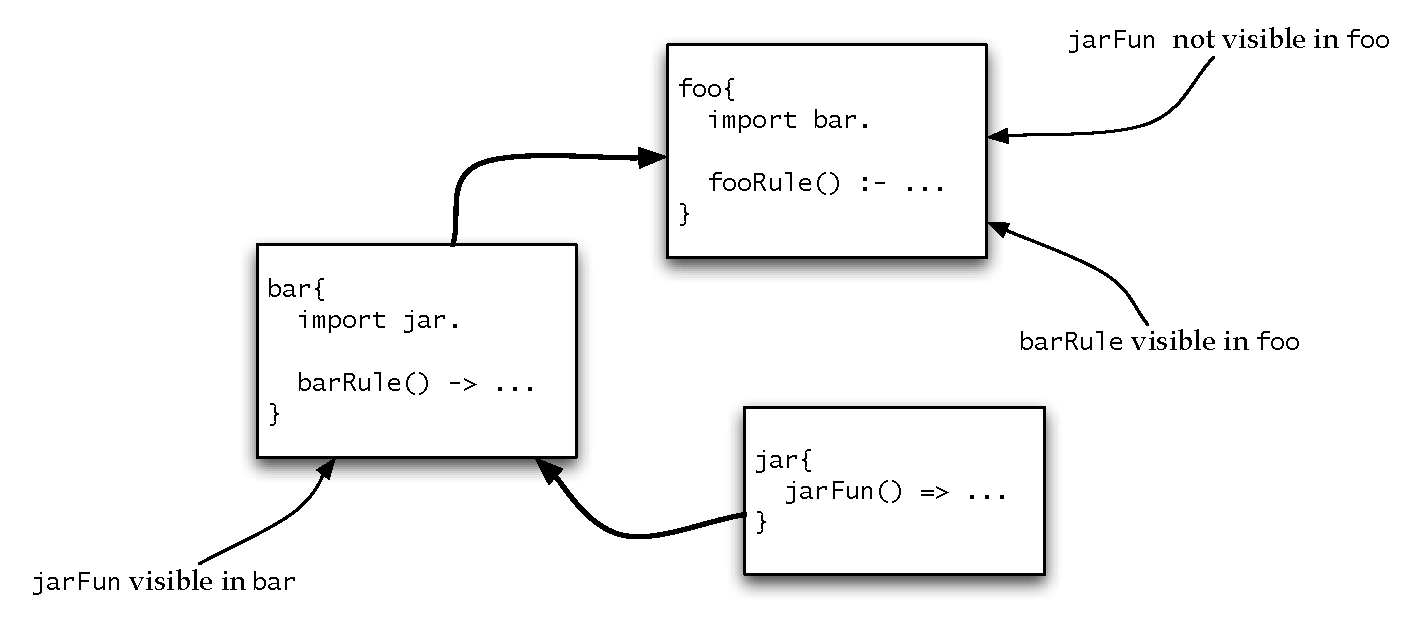
\includegraphics[width=\textwidth]{packages}
\caption{A three-way package \q{import}}
\label{program:packages:imports}
\end{figure}
It is possible for a package to \q{import} a package that, in turn, \q{import}s other packages. These latter packages will be automatically loaded as needed. However, the definitions in these dependent packages are \emph{not} automatically made available to the original \q{import}er. For example, figure~\vref{program:packages:imports} illustrates a case with three packages: \q{foo}, \q{bar} and \q{jar}.
In this scenario \q{jarFun} is available within the \q{bar} package, but not in the \q{foo} package -- even though loading the \q{foo} package will cause \q{jar} to be loaded. If \q{jarFun} is required directly within the \q{foo} then it will have to be explicitly \q{import}ed by the \q{foo} package. Of course, the \q{barRule} action procedure is available within the \q{foo} package.

This can become an issue for type and other definitions that are shared over many packages. In that situation, the shared definitions will need to be \q{import}ed in each context that they are required.

\begin{aside}
One workable technique, as used in our meta interpreter in Chapter~\ref{vmeta}, is to place commonly used types in a package of their own. Then, this type package may be \q{import}ed as needed.
\end{aside}

\index{circular chains of \q{import}s}
\index{package!recursive \q{import} not permitted}
\paragraph{Compiling packages}
The \go compiler requires that a package be compiled (see section~\vref{first:compiling}) before it can be imported; more specifically the compiler searches for the compiled package when compiling a package that \q{import}s a package. Thus, it may be important to ensure that dependent packages are compiled after the packages that they depend on. It is not permitted to have a circular chain of package \q{import}s -- with one package importing another, which in turn causes the original to be imported.

\subsection{Package reference}
\label{package:reference}
\index{operator!\#@\hash}
\index{package!reference}
\index{identifier!package reference}
There are occasions when it is necessary to identify \emph{which} package a particular identifier comes from. The primary purpose here is to resolve the situation where two packages export the \emph{same} identifier; in which case it is not defined which import is respected.

To precisely identify the package for a particular use, we use a \q{\hash} operator:
\begin{alltt}
go.io#stdout
\end{alltt}
The package name on the left is the name of the package -- as it is mentioned in the associated package \q{import} statement. The identifier on the right is one of the identifiers exported by the package.

\section{Top-level main programs}
\label{program:top-level}
Any package can also be treated as the top-level program -- provided that the package has a definition for the single argument action procedure \q{main}. In fact, \q{main} is a reserved keyword in \go: if a \q{main} program is defined in a package then it \emph{must} be consistent with the type assertion:
\begin{alltt}
main:(list[string])*
\end{alltt}
\index{main@\q{main} program}
\index{executing a \go program}

If a package is executed at the top-level, then the \q{main} program in that package is executed and given as its single argument a list of the command-line arguments specified in the execution. For example, if a package \q{foo} were mentioned as the top-level package to execute in:
\begin{alltt}
\% go foo a b c
\end{alltt}
then the package \q{foo} must have an appropriate definition for \q{main} and that action procedure is entered -- with argument the list
\begin{alltt}["a","b","c"]\end{alltt}
\begin{aside}
Since the command line arguments are passed in as \q{string}s it is common for these argument strings to be parsed before they can be used in the application proper.  

\index{operator!\%\%@\q{\%\%}}
The \q{\%\%} parse expression (see page~\pageref{expression:grammarexp}) and the \q{go.stdparse} package become handy in this situation. For example, to pass a numeric value to a \go fragment, where the number comes from the command line itself, then the classic way to do this is:
\begin{alltt}
mainPackage\{
  import go.stdparse.
  
  \ldots
  main([Arg,..More]) ->
    appProg(numeric\%\%Arg);\ldots
\}
\end{alltt}
The \q{numeric} grammar program parses a string into a \q{number} value.
\end{aside}

\section{Standard Packages}
\index{package!standard}
\index{standard packages}
Much of the functionality of the \go system is encapsulated in special packages that are distributed with the \go system. These are generally not automatically included in every program. By convention, all \go system packages have package names of the form: \q{go.\emph{name}}; for example, the system input/output package is called \q{go.io}. To access the standard I/O package, then, it is necessary to load the \q{go.io} package:
\begin{alltt}
\emph{yourpackage}\{
  import go.io.
  
  \ldots
\}
\end{alltt}
\begin{aside}
Input and output are, of course, fairly prevalent in programming. However, the reason that \q{go.io} is not automatically included in every package is that that permits non-standard I/O systems to be used - for example in embedded applications, or in systems which have to interact with file systems in special ways.
\end{aside}
The standard set of packages will vary from time to time, the current set includes the packages
\begin{description}
\item[\q{go.cell}] Implements a re-assignable resource entity.
\item[\q{go.datelib}] Implements a collection of date related functions.
\item[\q{go.dynamic}] Implements dynamic relations; relations that can be updated.
\item[\q{go.hash}] Implements a hash-table package.
\item[\q{go.io}] Implements the standard I/O package
\item[\q{go.mbox}] Implements an internal thread communication package.
\item[\q{go.setlib}] Implements a collection of set-like functions.
\item[\q{go.sort}] Implements a sort function
\item[\q{go.stack}] Implements a shareable updatable stack package.
\item[\q{go.queue}] Implements a shareable updatable queue package.
\item[\q{go.stdlib}] The standard \go language support package. This package is automatically loaded as it is required for successful execution of any \go program.
\item[\q{go.stdparse}] Implements a range of parsing functions, allowing the conversion of strings to numbers, for example.
\item[\q{go.unit}] Implements a unit-testing framework.
\item[\q{go.xml}] Implements an XML parser and displayer package. Also defines the \go version of the DOM (Document Object Model).
\item[\q{go.goweb}] A simple Web server written in \go.
\end{description}




